\documentclass[12pt]{article}
% begin font setup
\usepackage[T1]{fontenc}
\usepackage{mathptmx}
\usepackage[scaled=.92]{helvet}
\usepackage{courier}
% end font setup
% begin other packages
\usepackage{textcomp}
\usepackage[intlimits]{amsmath}
% end other packages
\usepackage{graphicx}
\usepackage{color}
\setlength{\paperwidth}{340bp}
\setlength{\paperheight}{206bp}
\pagestyle{empty}
\setlength{\voffset}{-1in}
\setlength{\topmargin}{0bp}
\setlength{\headheight}{0bp}
\setlength{\headsep}{0bp}
\setlength{\topskip}{0bp}
\setlength{\hoffset}{-1in}
\setlength{\oddsidemargin}{0bp}
\setlength{\evensidemargin}{0bp}
\setlength{\marginparwidth}{0bp}
\setlength{\marginparsep}{0bp}
\setlength{\textwidth}{\paperwidth}
\setlength{\textheight}{\paperheight}
\setlength{\parskip}{0bp}
\setlength{\parindent}{0bp}
\setlength{\pdfpagewidth}{\paperwidth}
\setlength{\pdfpageheight}{\paperheight}
\begin{document}%
\begin{picture}(0,0)
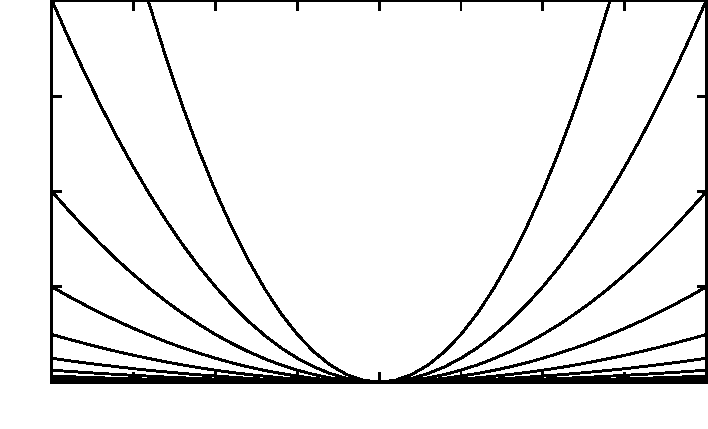
\includegraphics{ring-i.pdf}
\end{picture}%
\setlength{\unitlength}{1bp}%
\newfont{\FigToLatFontA}{ptmr at 10pt}%
\begin{picture}(340,206)
\put(51.875,148.045){\makebox(0,0)[lb]{\smash{{\color[rgb]{0,0,0}$R$=0.4}}}}
\put(30.815,66.025){\makebox(0,0)[lb]{\smash{{\color[rgb]{0,0,0}$R$=1.6}}}}
\put(33.155,106.525){\makebox(0,0)[lb]{\smash{{\color[rgb]{0,0,0}$R$=0.8}}}}
\put(82.655,178.525){\makebox(0,0)[lb]{\smash{{\color[rgb]{0,0,0}$R$=0.2}}}}
\put(0.455,113.965){\rotatebox{90.0174}{\makebox(0,0)[b]{\smash{{\color[rgb]{0,0,0}$h_U$ ($\mu$m)}}}}}
\put(181.955,0.085){\makebox(0,0)[b]{\smash{{\color[rgb]{0,0,0}$x_1$ ($\mu$m)}}}}
\put(339.095,11.305){\makebox(0,0)[b]{\smash{{\FigToLatFontA\color[rgb]{0,0,0}900}}}}
\put(299.795,11.305){\makebox(0,0)[b]{\smash{{\FigToLatFontA\color[rgb]{0,0,0}800}}}}
\put(260.555,11.305){\makebox(0,0)[b]{\smash{{\FigToLatFontA\color[rgb]{0,0,0}700}}}}
\put(221.255,11.305){\makebox(0,0)[b]{\smash{{\FigToLatFontA\color[rgb]{0,0,0}600}}}}
\put(182.015,11.305){\makebox(0,0)[b]{\smash{{\FigToLatFontA\color[rgb]{0,0,0}500}}}}
\put(142.715,11.305){\makebox(0,0)[b]{\smash{{\FigToLatFontA\color[rgb]{0,0,0}400}}}}
\put(103.415,11.305){\makebox(0,0)[b]{\smash{{\FigToLatFontA\color[rgb]{0,0,0}300}}}}
\put(64.175,11.305){\makebox(0,0)[b]{\smash{{\FigToLatFontA\color[rgb]{0,0,0}200}}}}
\put(24.875,11.305){\makebox(0,0)[b]{\smash{{\FigToLatFontA\color[rgb]{0,0,0}100}}}}
\put(20.375,201.745){\makebox(0,0)[rb]{\smash{{\FigToLatFontA\color[rgb]{0,0,0}20}}}}
\put(20.375,156.025){\makebox(0,0)[rb]{\smash{{\FigToLatFontA\color[rgb]{0,0,0}15}}}}
\put(20.375,110.305){\makebox(0,0)[rb]{\smash{{\FigToLatFontA\color[rgb]{0,0,0}10}}}}
\put(20.375,64.525){\makebox(0,0)[rb]{\smash{{\FigToLatFontA\color[rgb]{0,0,0}5}}}}
\put(20.375,18.805){\makebox(0,0)[rb]{\smash{{\FigToLatFontA\color[rgb]{0,0,0}0}}}}
\end{picture}%
\end{document}
